\documentclass[final]{beamer}
\mode<presentation>
{
  \usetheme{JDM}
}

\usepackage{multirow}
\usepackage{ragged2e}
\usepackage{times}
\usepackage{amsmath,amssymb}
\usepackage[english]{babel}
\usepackage[latin1]{inputenc}
\usepackage[orientation=landscape, size=custom, width=84, height=118, scale=1]{beamerposter}
\usepackage{array}
\usepackage{xspace}
\usepackage{xcolor}
\usepackage{epsfig}
\usepackage{caption}
\usepackage{subcaption}
\usepackage{booktabs}
\usepackage{wrapfig}

\newcommand{\iqadataset}{\mbox{IQA}}
\newcommand{\thornav}{\mbox{IQA}}

\DeclareMathAlphabet\mathbfcal{OMS}{cmsy}{b}{n}

% Relations.
\newcommand{\IN}{\textit{in}}
\newcommand{\ON}{\textit{on}}

% Objects in pair.
\newcommand{\grasped}{$O_G$}
\newcommand{\target}{$O_T$}

% Models.
\newcommand{\ego}[1]{$M^{\mathrm{ego}}_{#1}$}
\newcommand{\obj}[1]{$M^{\mathrm{obj}}_{#1}$}
\newcommand{\egoobj}[1]{$M^{\mathrm{ego+obj}}_{#1}$}
\newcommand{\egoPobj}[1]{$M^{\mathrm{ego+pre}}_{#1}$}
\newcommand{\Pobj}[1]{$M^{\mathrm{pre}}_{#1}$}

% Zero vector.
\newcommand{\zv}{$\textcolor{red}{\vec{0}}$}

\usepackage{soul}
\usepackage{xcolor}
\usepackage{colortbl}
\usepackage{pifont}
\usepackage{multirow}  % added

% Poster text sizes.
\newcommand{\setblocksize}{\LARGE \centering}
\newcommand{\setsize}{\Large}
\newcommand{\setcentersize}{\LARGE}
\newcommand{\paragraphbreak}{\vspace{1cm}}
\newcommand{\sidecolumnwidth}{.22}
\newcommand{\centercolumnwidth}{.49}

\newcommand{\datasetfull}{Cooperative Vision-and-Dialog Navigation}
\newcommand{\dataset}{CVDN}
\newcommand{\taskfull}{Navigation from Dialog History}
\newcommand{\task}{NDH}

\newcommand{\cblkmark}{\ding{51}}
\newcommand{\cmark}{\color{blue}{\ding{51}}}
\newcommand{\xmark}{\color{red}{\ding{55}}}
\newcommand{\good}[1]{\textcolor{blue}{\textbf{#1}}}
\newcommand{\bad}[1]{\textcolor{red}{\textbf{#1}}}
\newcommand{\neutral}[1]{\textcolor{purple}{\textbf{#1}}}

\newcommand{\nav}{\textit{Navigator}}
\newcommand{\ora}{\textit{Oracle}}

\title{Vision-and-Dialog Navigation}
\author{Jesse Thomason, Michael Murray, Maya Cakmak, Luke Zettlemoyer}
\institute{{\texorpdfstring{\color{blue} \bf \huge}{ }Jesse Thomason}\hspace{1em} {\texorpdfstring{\color{blue} \bf \huge}{ }Michael Murray} \\ Maya Cakmak\hspace{1em} Luke Zettlemoyer\\University of Washington}

\date{\today}

\begin{document}
\setbeamertemplate{caption}{\raggedright\insertcaption\par}
%%%%%%%%%%%%%%%%%%%%%%%%%%%%%%%%%%%%%%%%%%%%%%%%%%%%%%%%%%%%%%%%%%%%%%%%%%%%%%%%%%%%%%%%%%%
\begin{frame}{} 
  \vfill
  
%\vspace{-270pt}  %added here to get it closer to top...
\begin{columns}[t]

%%%%%%%%%%%%%%%%%%%%%%%%%%%%%%%%%%%%%%%%%%%%%%%%%%%%%%%%%%%%%%%%%%%%%%%%%%%%%%%%%%%%%%%%%%%
\begin{column}{\sidecolumnwidth\linewidth}    %%% COLUMN 1 %%%

\begin{block}{\setblocksize Contributions}
%\vspace{-30pt}
	\vspace{1mm}
\justifying{\setsize

\begin{itemize}
  \item[+] Over 2k human-human navigation dialogs.
  \item[+] Initial navigation models.
  \item[+] Dialog helps navigation.
  \item[+] Mixed human and planner supervision helps.
  \item[+] Navigation challenge leaderboard.
\end{itemize}

}
\end{block}

\begin{block}{\setblocksize Dataset}
  \vspace{1mm}
\justifying{\setsize

\dataset{} is the first dataset to include two-sided dialogs held in natural language, with the initial navigation instruction being both ambiguous (\textit{Amb}) and underspecified (\textit{UnderS}), and situated in a photorealistic, visual navigation environment viewed by both speakers.

\begin{table}[ht!]
\centering
\begin{tiny}
\begin{tabular}{lccccccc}
    \textbf{Dataset} & \multicolumn{4}{c}{\textbf{---Language Context---}} & \multicolumn{3}{c}{\textbf{---Visual Context---}} \\
    & Human & Amb & UnderS & Temporal & Real-world & Temporal & Shared \\
    \toprule
MARCO\cite{macmahon:aaai06,chen:aaai11}, DRIF\cite{blukis:corl18} & \cmark & \xmark & \xmark & \bad{1I} & \xmark & \good{Dynamic} & - \\
    R2R\cite{anderson:cvpr18}, Touchdown\cite{chen:cvpr19} & \cmark & \xmark & \xmark & \bad{1I} & \cmark & \good{Dynamic} & - \\
    EQA\cite{das:cvpr18}, IQA\cite{gordon2018iqa} & \xmark & \xmark & \cmark & \bad{1Q} & \xmark & \good{Dynamic} & - \\
    CLEVR\cite{johnson:cvpr17} & \xmark & \xmark & - & \bad{1Q} & \xmark & \bad{Static} & - \\
    VQA\cite{antol:iccv15,hudson:cvpr18,zellers:cvpr19} & \cmark & \xmark & - & \bad{1Q} & \cmark & \bad{Static} & - \\
    CLEVR-Dialog\cite{kottur:naacl19} & \xmark & \xmark & - & \good{2D} & \xmark & \bad{Static} & \cmark \\
    VisDial\cite{das:cvpr17} & \cmark & \xmark & - & \good{2D} & \cmark & \bad{Static} & \cmark \\
    VLNA\cite{nguyen:cvpr19}, HANNA\cite{nguyen:emnlp19} & \xmark & \cmark & \cmark & \neutral{1D} & \cmark & \good{Dynamic} & \xmark \\
    TtW\cite{devries:arxiv18} & \cmark & \xmark & \cmark & \good{2D} & \cmark & \good{Dynamic} & \xmark \\
    \midrule
    \dataset{} & \cmark & \cmark & \cmark & \good{2D} & \cmark & \good{Dynamic} & \cmark \\
    \bottomrule
\end{tabular}
\end{tiny}
\end{table}

Human \nav{} paths are longer than shortest path planner routes, resulting in much longer paths than in the comparable Room-to-Room dataset.

\begin{figure}[ht]
\begin{tabular}{cc}
    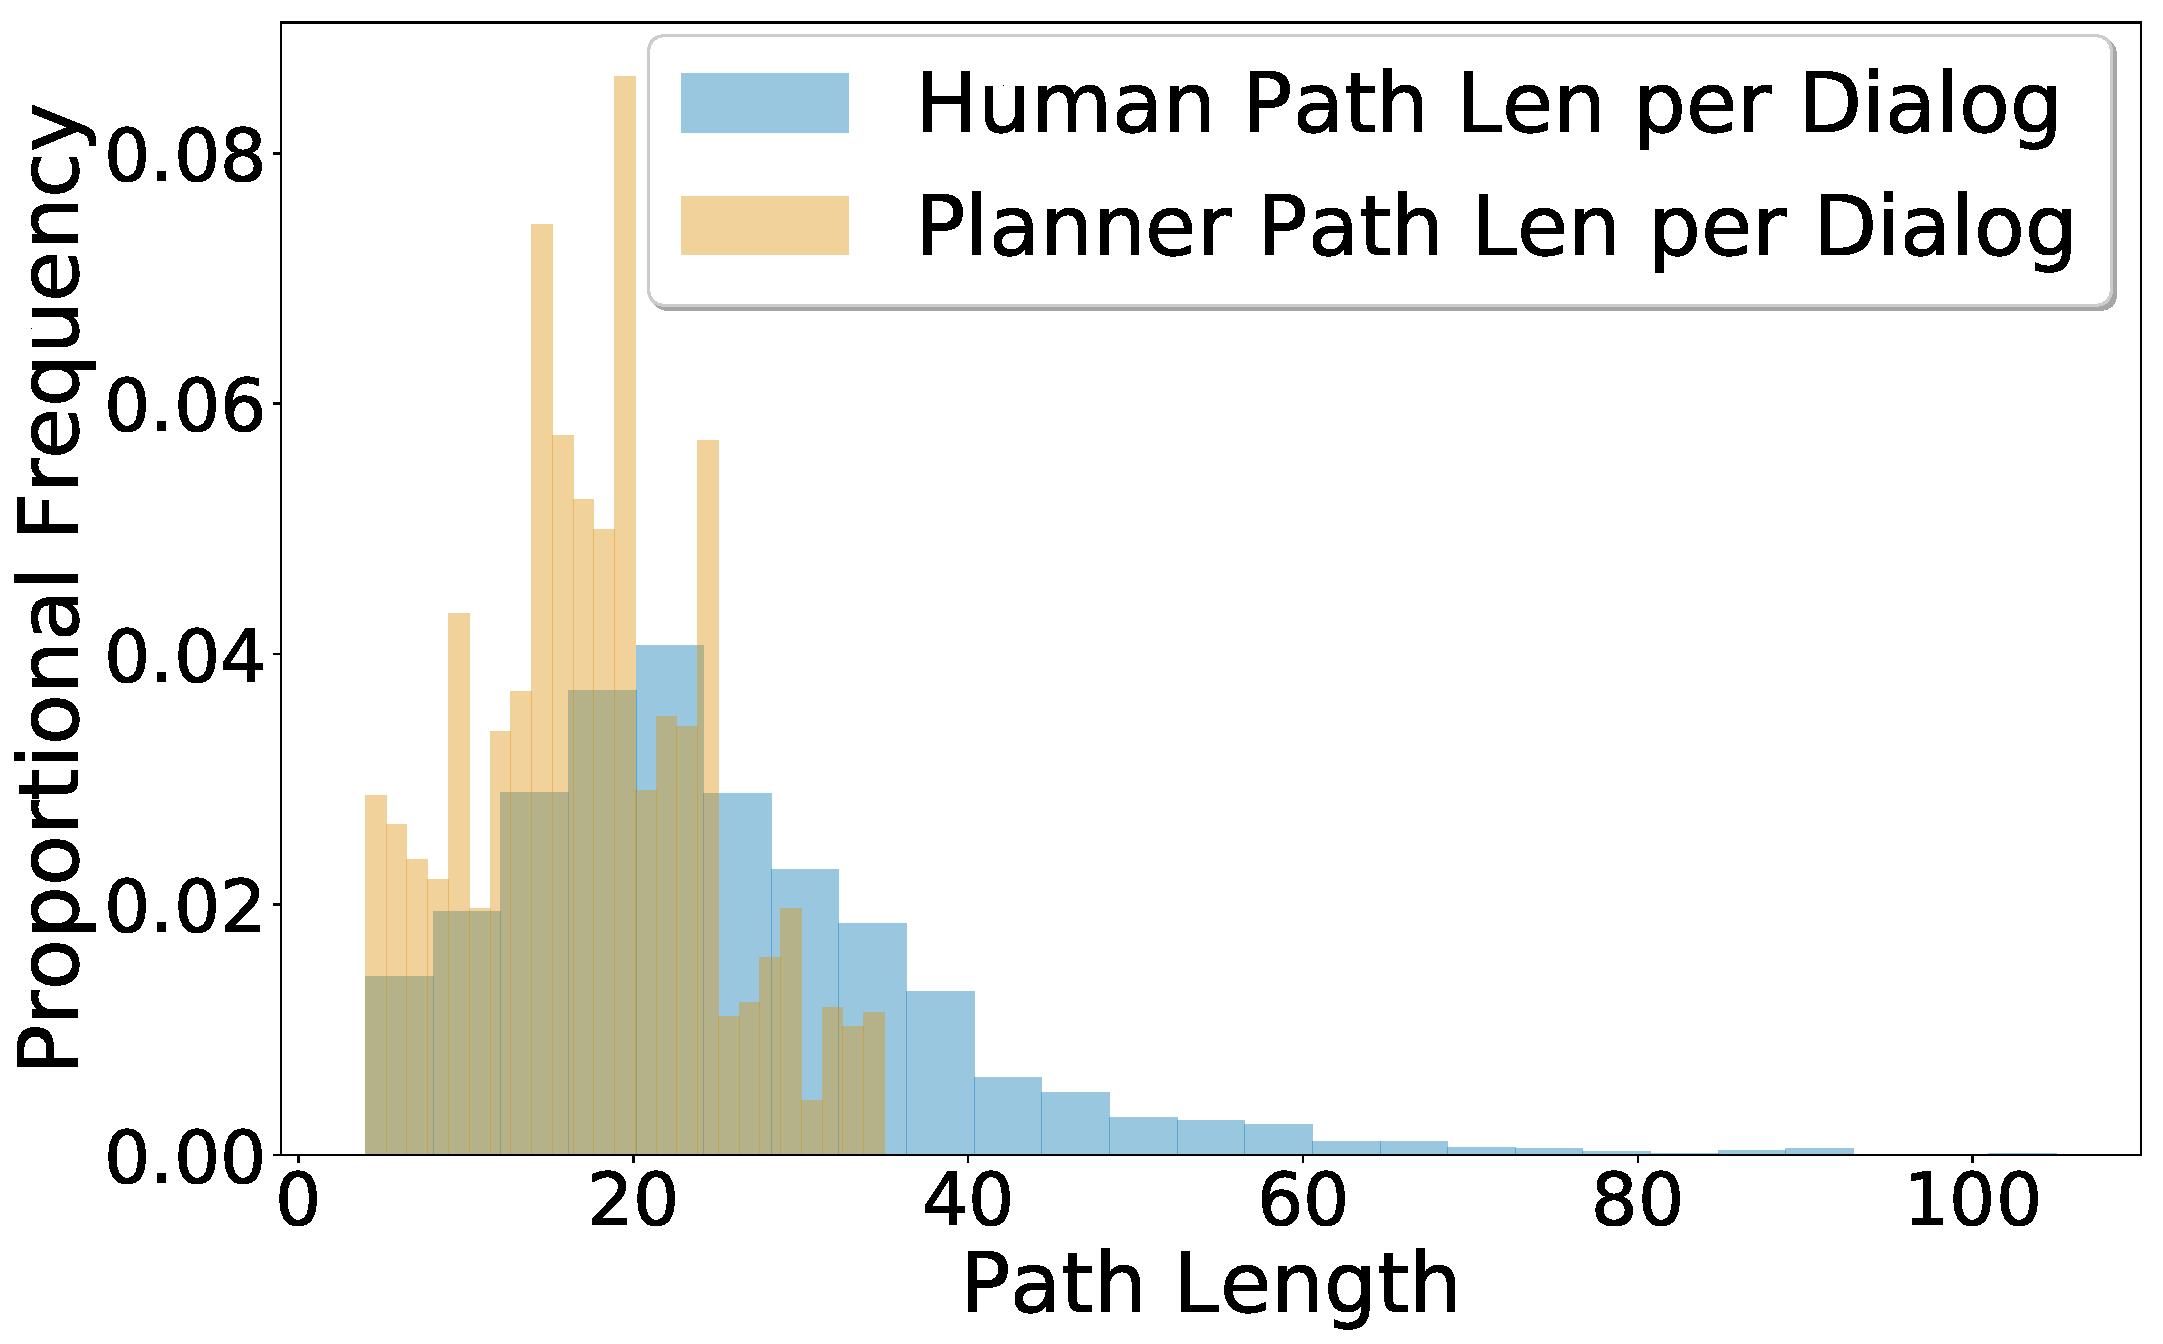
\includegraphics[width=0.45\columnwidth]{figures/player_planner_steps_per_dialog.pdf} &
    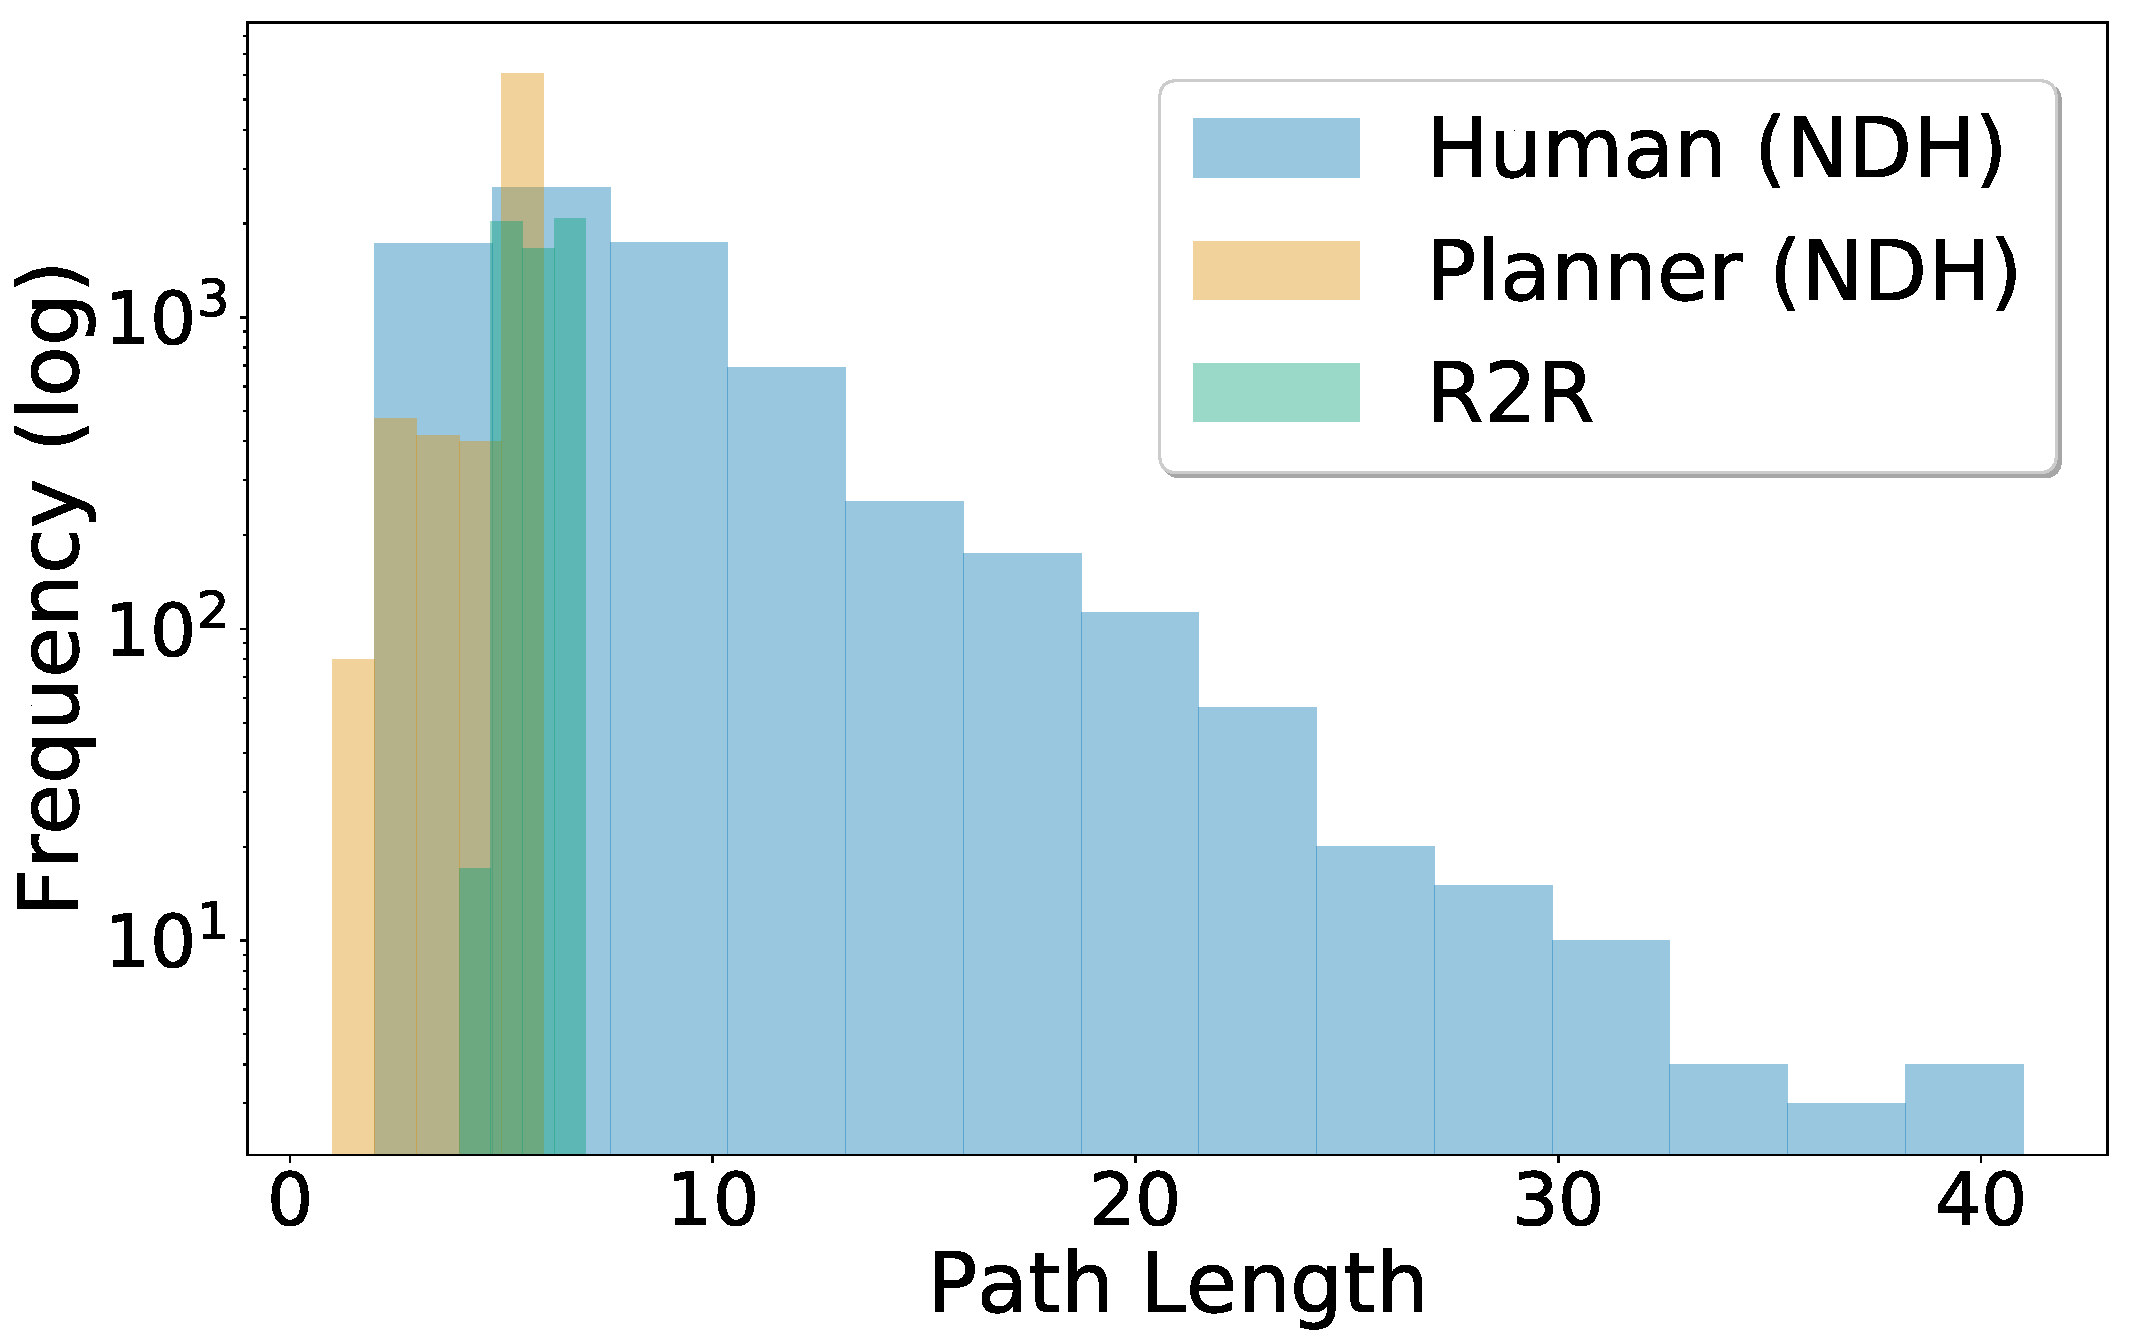
\includegraphics[width=0.45\columnwidth]{figures/path_len_per_ndh.pdf} \\
    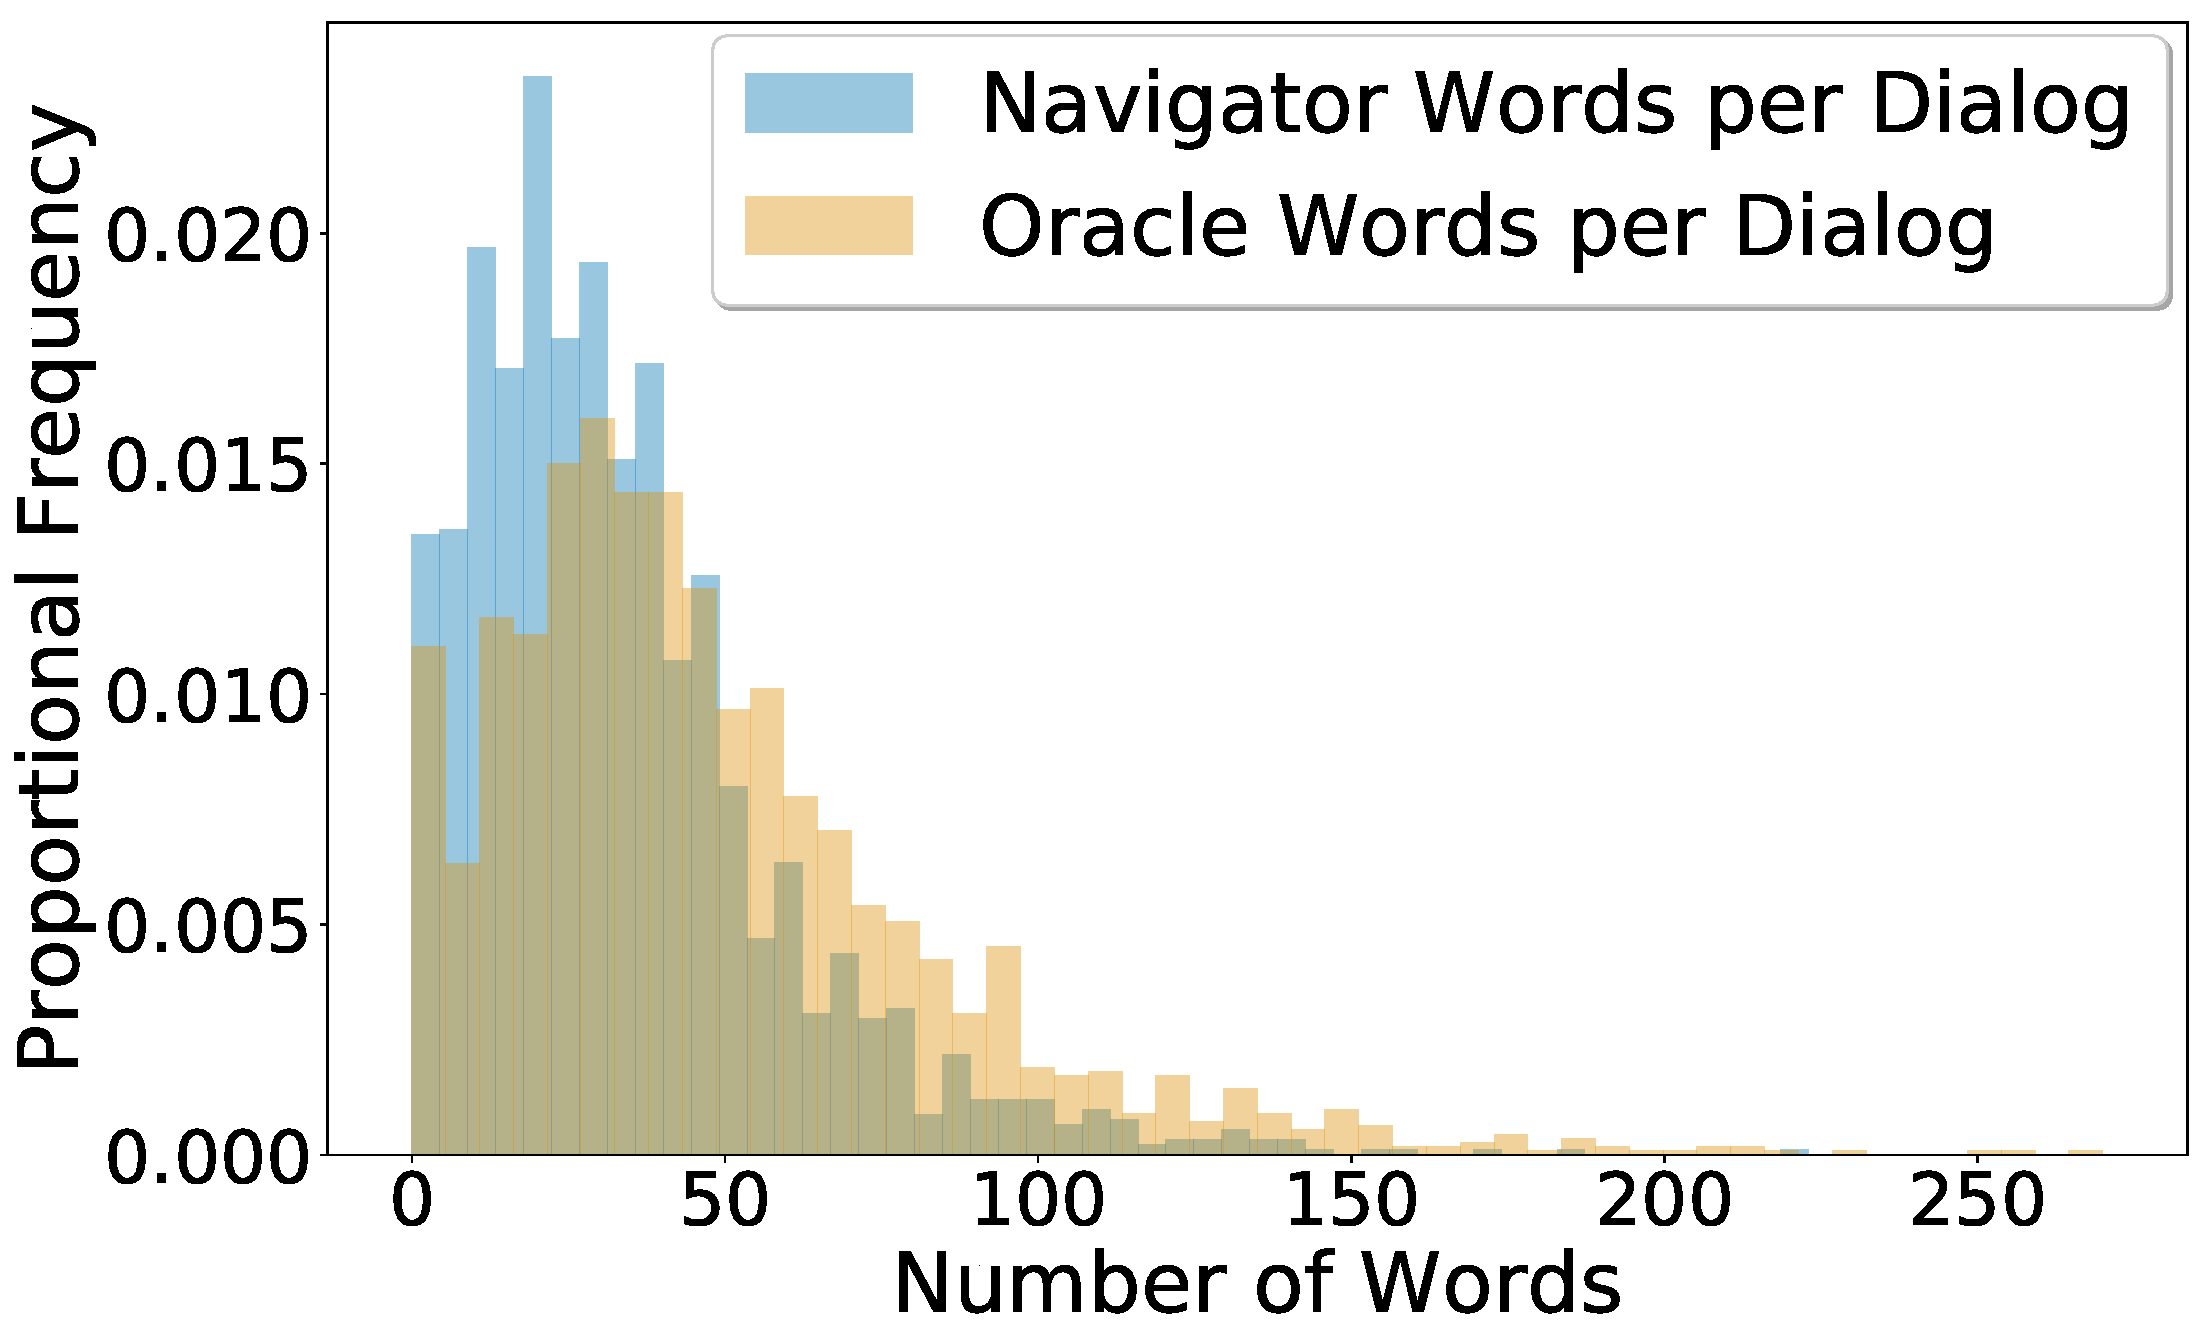
\includegraphics[width=0.45\columnwidth]{figures/nav_ora_words_per_dialog.pdf} &
    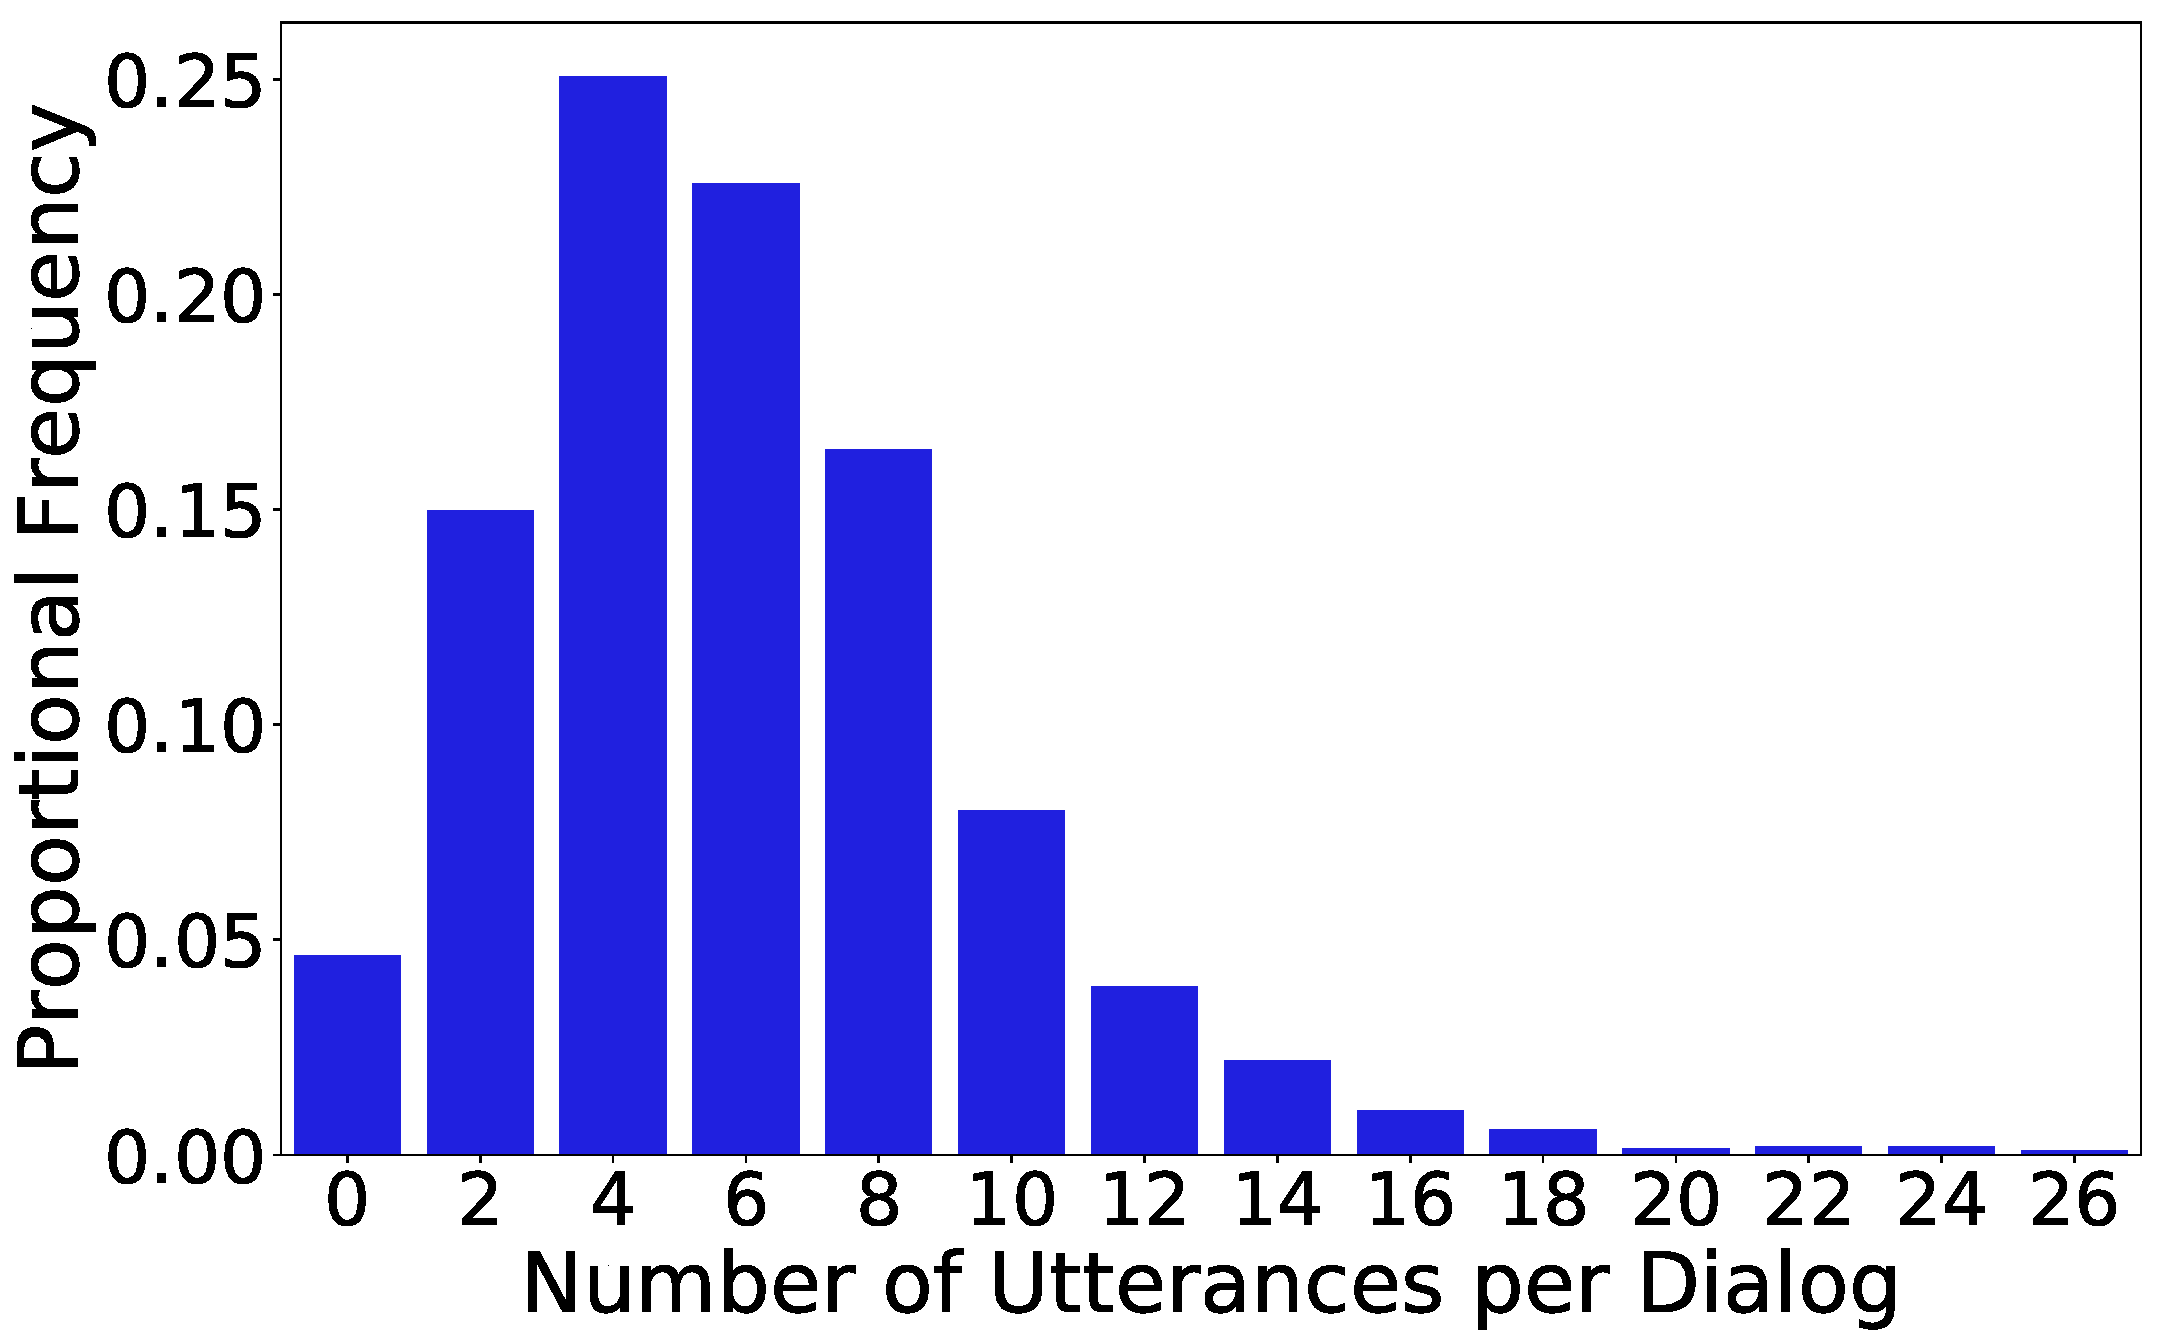
\includegraphics[width=0.45\columnwidth]{figures/utterances_per_dialog.pdf}
\end{tabular}
\vspace{-4mm}
\end{figure}

Human \ora{}s use more words than \nav{}s, and dialogs have on average 3-4 question-answer exchanges each.

\begin{table}[ht]
\centering
\begin{footnotesize}
\begin{tabular}{p{2cm}rrrp{10cm}}
    & \textbf{\textit{Dia}} & \textbf{\textit{Nav}} & \textbf{\textit{Ora}} & \textbf{Example} \\
    \toprule
    Ego & $92.5$ & $52.9$ & $65.8$ & \ora{}: Turn slightly to {\color{blue}your right} and go {\color{blue}forward} down the hallway \\
    \cmidrule{5-5}
    Needs Q & $13.0$ & - & $3.9$ & \nav{}: Should I turn left down the hallway ahead? \\
    & & & &  \ora{}: {\color{blue}ya} \\
    \cmidrule{5-5}
    Needs Dialog History & $3.5$ & $0.4$ & $1.0$ & \ora{}: Through the lobby. So go through the door next to the green towel. Go to the left door next to {\color{blue}the two yellow lights}. Walk straight to the end of the hallway and stop \\
    & & & & $\dots$ \\
    & & & & \nav{}: Are these {\color{blue}the yellow lights} you were talking about? \\
    \cmidrule{5-5}
    Needs Nav History & $14.0$ & $1.5$ & $3.4$ & \ora{}: {\color{blue}You were there briefly but left}. There is a turntable behind you a bit. Enter the bedroom next to it. \\
    \cmidrule{5-5}
    Repair & $12.5$ & $1.6$ & $3.4$ & \ora{}: I am so sorry {\color{blue}I meant for you to look over to the right not the left} \\
    \cmidrule{5-5}
    Off-topic & $3.0$ & $5.4$ & $5.1$ & \nav{}: I am to the `rear' of the zebra. {\color{blue}Nice one.} \\
    & & & & \ora{}: {\color{blue}Ok hold your nose} and go to the left of the zebra, through the livingroom and kitchen and towards the bedroom you can see past that \\
    \cmidrule{5-5}
    Vacuous & $6.0$ & $22.7$ & $2.3$ & \nav{}: {\color{blue}Ok, now where?} \\
    \bottomrule \\
\end{tabular}
\end{footnotesize}
\vspace{-8mm}
\end{table}
The average percent of \textit{Dialogs}, as well as individual \nav{} and \ora{} utterances, exhibiting each phenomena out of 100 hand-annotated dialogs.

}
\end{block}

\end{column}	%%% END COLUMN 1 %%%

%%%%%%%%%%%%%%%%%%%%%%%%%%%%%%%%%%%%%%%%%%%%%%%%%%%%%%%%%%%%%%%%%%%%%%%%%%%%%%%%%%%%%%%%%%%
\begin{column}{\centercolumnwidth\linewidth}    %%% COLUMN 2 %%%

\setbeamercolor*{block body}{bg=uwmetal,fg=white}
\begin{block}{\setblocksize \datasetfull{} (\dataset{})}
  \vspace{1mm}
\justifying{\Huge
\begin{itemize}
\item[] A big dataset of human-human dialogs!
\item[] Training navigation agents!
\item[] A demo interface! $\Downarrow$
\end{itemize}
}

\begin{figure}
  \centering
  
\includegraphics[width=0.3\linewidth]{QR.png}
\end{figure}

\end{block}
\setbeamercolor*{block body}{bg=white,fg=black}



\begin{block}{\setblocksize }
  \vspace{1mm}
\justifying{\setcentersize

\begin{figure}[!t]
  \centering
  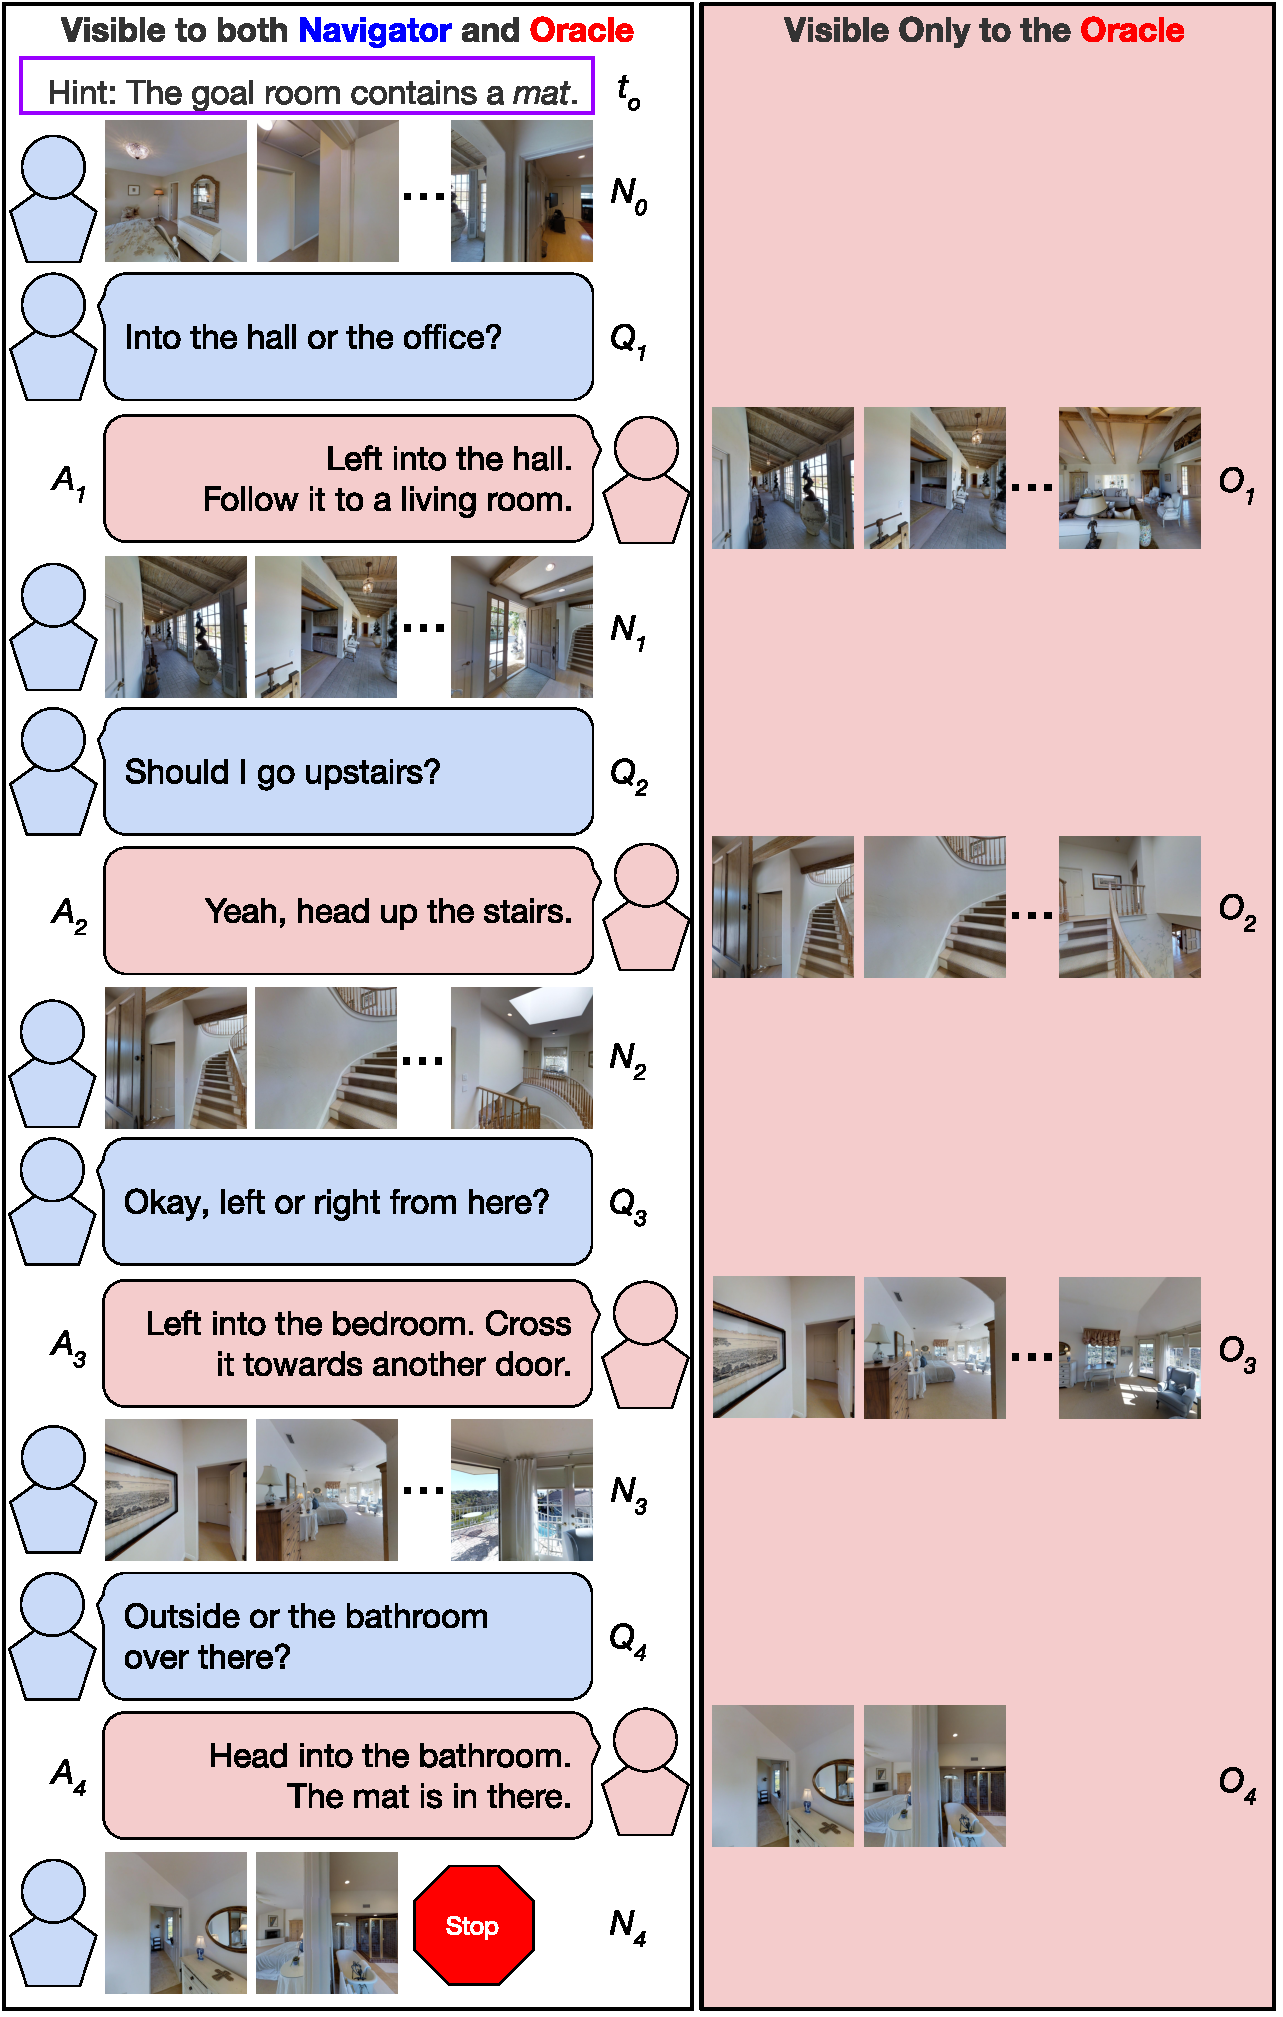
\includegraphics[width=0.95\linewidth]{figures/full_demo_vertical.pdf}
\end{figure}

\begin{figure}
  \centering
  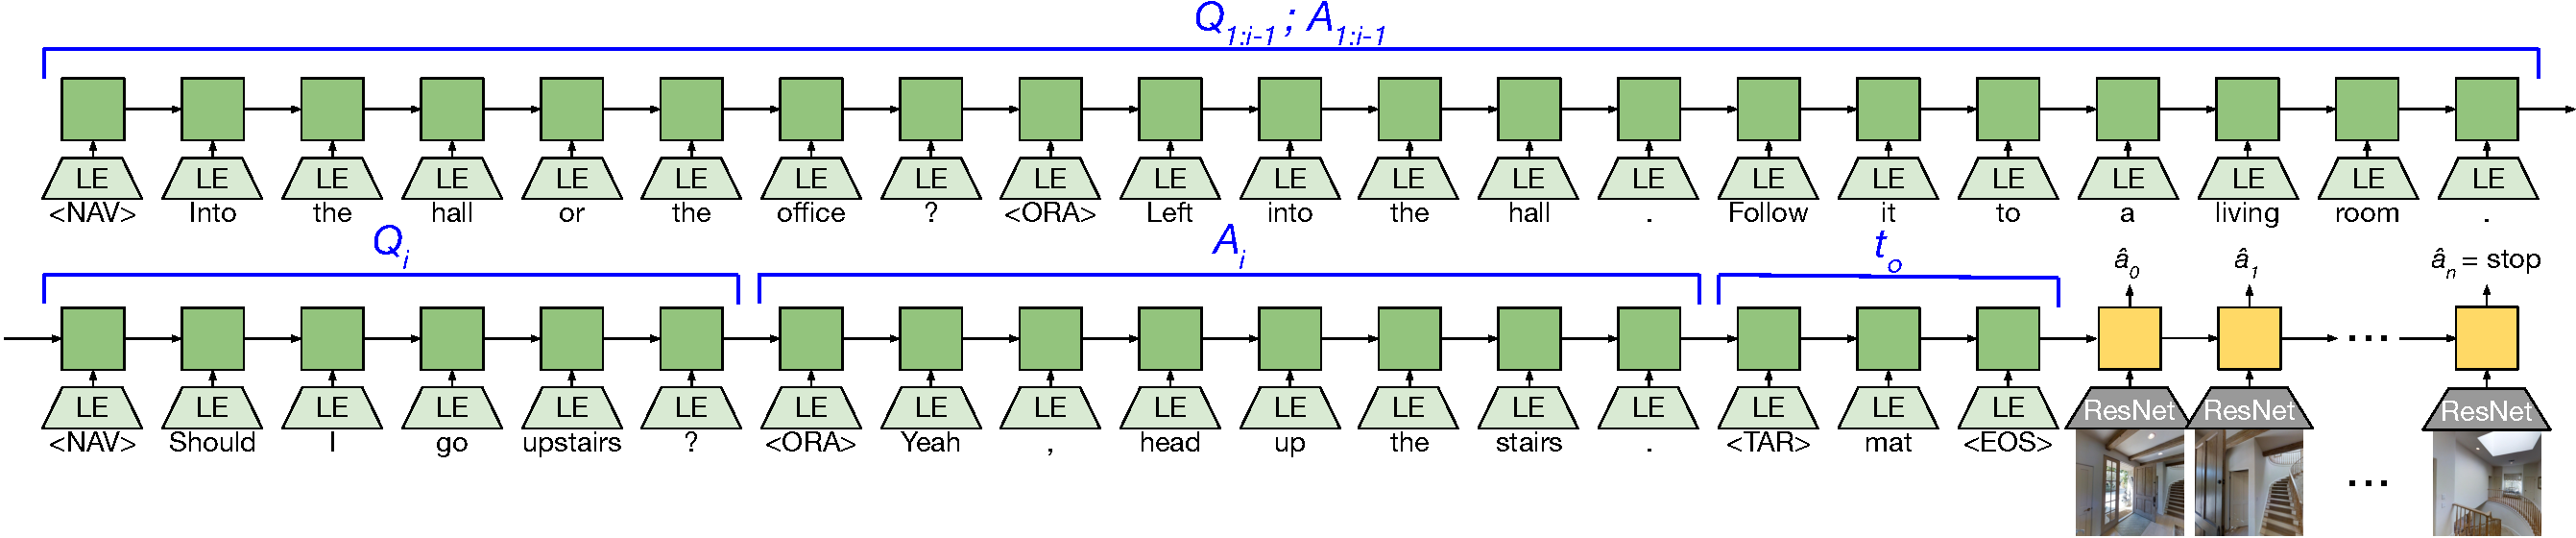
\includegraphics[width=\linewidth]{figures/model.pdf}    
\end{figure}

}
\end{block}

\end{column}  %%% END COLUMN 2 %%%

%%%%%%%%%%%%%%%%%%%%%%%%%%%%%%%%%%%%%%%%%%%%%%%%%%%%%%%%%%%%%%%%%%%%%%%%%%%%%%%%%%%%%%%%%%%
\begin{column}{\sidecolumnwidth\linewidth}    %%% COLUMN 3 %%%

\begin{block}{\setblocksize Navigation Task}
  \vspace{1mm}
\justifying{\setsize

For each question-answer exchange, we task an agent with navigating towards the goal given the dialog so far.
We can use the path taken by the \nav{}, shown to the \ora{}, or a \emph{mix} as supervision.

}
\end{block}

\begin{block}{\setblocksize Evaluation}
	\vspace{1mm}
\justifying{\setsize

Average agent progress towards the goal location when trained using different path end nodes for supervision.
Among ablations, \textbf{bold} indicates most progress by language input, and \good{blue} indicates most progress by supervision signal.

\begin{table}[ht]
\centering
\begin{small}
\begin{tabular}{ccccccc>{\raggedleft\arraybackslash}p{2.6cm}>{\raggedleft\arraybackslash}p{2.6cm}>{\raggedleft\arraybackslash}p{2.6cm}}
    & & \multicolumn{5}{c}{\textbf{Seq-2-Seq Inputs}} & \multicolumn{3}{c}{\textbf{Goal Progress} (m) $\uparrow$} \\
    & & & & & & $Q_{1:i-1} $ & & & \\
    \textbf{Fold} & & $V$ & $t_o$ & $A_i$ & $Q_i$ & $A_{1:i-1}$ & \textbf{Oracle} & \textbf{Navigator} & \textbf{Mixed} \\
\toprule
    \multirow{9}{*}{\rotatebox[origin=c]{90}{Val (Seen)}} & \multirow{5}{*}{\rotatebox[origin=c]{90}{Baselines}} & \multicolumn{5}{c}{\texttt{Shortest Path}} & $8.29$ & $7.63$ & $9.52$ \\
    & & \multicolumn{5}{c}{\texttt{Random}} & $0.42$ & $0.42$ & $0.42$ \\
    & & & & & & & $0.59$ & $0.83$ & $0.91$ \\
    & & \cblkmark & & & & & $4.12$ & $5.58$ & $5.72$ \\
    & & & \cblkmark & \cblkmark  & \cblkmark  & \cblkmark & $1.41$ & $1.43$ & $1.58$ \\
    \cmidrule{2-10}
    & \multirow{4}{*}{\rotatebox[origin=c]{90}{Ours}} & \cblkmark & \cblkmark & & & & $4.16$ & \good{$\pmb{5.71}$} & \good{$5.71$} \\
    & & \cblkmark & \cblkmark & \cblkmark & & & $4.34$ & $5.61$ & \good{$6.04$} \\
    & & \cblkmark & \cblkmark & \cblkmark & \cblkmark & & $4.28$ & $5.58$ & \good{$\pmb{6.16}$} \\
    & & \cblkmark & \cblkmark & \cblkmark & \cblkmark & \cblkmark & $\pmb{4.48}$ & $5.67$ & \good{$5.92$} \\
    \midrule
    \multirow{9}{*}{\rotatebox[origin=c]{90}{Val (Unseen)}} & \multirow{5}{*}{\rotatebox[origin=c]{90}{Baselines}} & \multicolumn{5}{c}{\texttt{Shortest Path}} & $8.36$ & $7.99$ & $9.58$ \\
    & & \multicolumn{5}{c}{\texttt{Random}} & $1.09$ & $1.09$ & $1.09$ \\
    & & & & & & & $0.69$ & $1.32$ & $1.07$ \\
    & & \cblkmark & & & & & $0.85$ & $1.38$ & $1.15$ \\
    & & & \cblkmark & \cblkmark & \cblkmark & \cblkmark & $1.68$ & $1.39$ & $1.64$ \\
    \cmidrule{2-10}
    & \multirow{4}{*}{\rotatebox[origin=c]{90}{Ours}} & \cblkmark & \cblkmark & & & & $0.74$ & \good{$1.33$} & $1.29$ \\
    & & \cblkmark & \cblkmark & \cblkmark & & & $1.14$ & $1.62$ & \good{$2.05$} \\
    & & \cblkmark & \cblkmark & \cblkmark & \cblkmark & & $1.11$ & $1.70$ & \good{$1.83$} \\
    & & \cblkmark & \cblkmark & \cblkmark & \cblkmark & \cblkmark & $\pmb{1.23}$ & $\pmb{1.98}$ & \good{$\pmb{2.10}$} \\
    \midrule
    \multirow{9}{*}{\rotatebox[origin=c]{90}{Test (Unseen)}} & \multirow{5}{*}{\rotatebox[origin=c]{90}{Baselines}} & \multicolumn{5}{c}{\texttt{Shortest Path}} & $8.06$ & $8.48$ & $9.76$ \\
    & & \multicolumn{5}{c}{\texttt{Random}} & $0.83$ & $0.83$ & $0.83$ \\
    & & & & & & & $0.13$ & $0.80$ & $0.52$ \\
    & & \cblkmark & & & & & $0.99$ & $1.56$ & $1.74$ \\
    & & & \cblkmark & \cblkmark  & \cblkmark  & \cblkmark  & $1.51$ & $1.20$ & $1.40$ \\
    \cmidrule{2-10}
    & \multirow{4}{*}{\rotatebox[origin=c]{90}{Ours}} & \cblkmark & \cblkmark & & & & $1.05$ & $1.81$ & \good{$1.90$} \\
    & & \cblkmark & \cblkmark & \cblkmark & & & $1.21$ & $2.01$ & \good{$2.05$} \\
    & & \cblkmark & \cblkmark & \cblkmark & \cblkmark & & $\pmb{1.35}$ & $1.78$ & \good{$2.27$} \\
    & & \cblkmark & \cblkmark & \cblkmark & \cblkmark & \cblkmark & $1.25$ & $\pmb{2.11}$ & \good{$\pmb{2.35}$} \\
    \bottomrule \\
\end{tabular}
\end{small}
\vspace{-7mm}
\end{table}

Using all dialog history significantly outperforms unimodal ablations in \textit{unseen} environments.
Using all dialog history, rather than just the last question or question-answer exchange, is needed to achieve statistically significantly better performance than using the target object alone in \textit{unseen} test environments.
Dialog history is beneficial for understanding the context of the latest navigation instruction $A_i$.
Models trained with mixed supervision always statistically significantly outperform those trained with oracle or navigator supervision.
Using human demonstrations only when they appear trustworthy increases agent progress towards the goal.

}
\end{block}

\end{column}	%%% END COLUMN 3 %%%

%%%%%%%%%%%%%%%%%%%%%%%%%%%%%%%%%%%%%%%%%%%%%%%%%%%%%%%%%%%%%%%%%%%%%%%%%%%%%%%%%%%%%%%%%%%%%%%%%%%%
\end{columns}

\end{frame}

\end{document}


%%%%%%%%%%%%%%%%%%%%%%%%%%%%%%%%%%%%%%%%%%%%%%%%%%%%%%%%%%%%%%%%%%%%%%%%%%%%%%%%%%%%%%%%%%%%%%%%%%%%
%%% Local Variables: 
%%% mode: latex
%%% TeX-PDF-mode: t

